\documentclass[final,3p,times]{elsarticle}

\usepackage{lipsum}
 \usepackage{graphics}
\usepackage[]{algorithm2e}
 \usepackage{setspace}
%% or use the graphicx package for more complicated commands
 \usepackage{graphicx}
%% or use the epsfig package if you prefer to use the old commands
 \usepackage{epsfig}
 \usepackage{subfigure}

%% The amssymb package provides various useful mathematical symbols
\usepackage{amssymb}
%% The amsthm package provides extended theorem environments
 \usepackage{amsthm,amsmath}
 \usepackage{multirow}
 \usepackage{setspace}
 \usepackage{CJK}
 \usepackage{float}
 \usepackage{pdfpages}
 \restylefloat{table}
 \onehalfspacing



\makeatletter
\def\ps@pprintTitle{%
	\let\@oddhead\@empty
	\let\@evenhead\@empty
	\def\@oddfoot{}%
	\let\@evenfoot\@oddfoot}
\makeatother


\begin{document}

\begin{frontmatter}

\title{MATH 6740: Financial Mathematics and Simulation\\
	Homework 2 solutions/presentation}

\author[rvt]{Jubiao ``Jack'' Yang}

\address[rvt]{Rensselaer Polytechnic Institute, Troy, NY 12180}


\end{frontmatter}

\section{Q1}
	For each time interval $\Delta t$, the stock price's transition from $S(n)$ to $S(n+1)$ is based on a binary model, with $S(n+1)=uS(n)$ at probability $p_u$, and $S(n+1)=dS(n)$ at probability $p_d$. The coefficients $u$ and $d$ are:
	\begin{equation}
		\begin{cases}
			u=e^{\mu \Delta t + \sigma \sqrt{\Delta t}} ,\\
			d=e^{\mu \Delta t - \sigma \sqrt{\Delta t}} ,
		\end{cases}
	\end{equation}
	where $\mu$ and $\sigma$ are the mean rate of return per unit time and variance per unit time respectively. Under the assumption that the market is arbitrage-free, the probability of up and down-market are:
	\begin{subequations}
		\begin{equation}
			\begin{split}
				q_u &= \frac{e^{r\Delta t}-e^{\mu \Delta t - \sigma \sqrt{\Delta t}}}{e^{\mu \Delta t + \sigma \sqrt{\Delta t}} - e^{\mu \Delta t - \sigma \sqrt{\Delta t}}} \\
				&\approx \frac{r\Delta t + \frac{\left(r\Delta t\right)^2}{2}-\left[\mu\Delta t - \sigma\sqrt{\Delta t} + \frac{\left(\mu\Delta t - \sigma\sqrt{\Delta t}\right)^2}{2}\right]}{\left[\mu\Delta t + \sigma\sqrt{\Delta t} + \frac{\left(\mu\Delta t + \sigma\sqrt{\Delta t}\right)^2}{2}\right] - \left[\mu\Delta t - \sigma\sqrt{\Delta t} + \frac{\left(\mu\Delta t - \sigma\sqrt{\Delta t}\right)^2}{2}\right]} \\
				&= \frac{\left(r-\mu\right)\sqrt{\Delta t}+\frac{r^2}{2}\left(\Delta t\right)^{\frac{3}{2}} + \sigma - \frac{\mu^2\left(\Delta t\right)^{\frac{3}{2}} + \sigma^2 \sqrt{\Delta t} - 2\mu\sigma \Delta t }{2} }{2\sigma + 2\mu\sigma\Delta t} \\
				&\approx \frac{1}{2} + \frac{r-\mu-\frac{\sigma^2}{2}}{2\sigma} \sqrt{\Delta t}
				,
			\end{split}
		\end{equation}
		\begin{equation}
			q_d = 1 - q_u = \frac{1}{2} - \frac{r-\mu-\frac{\sigma^2}{2}}{2\sigma} \sqrt{\Delta t}
			.
		\end{equation}
	\end{subequations}
	Since $X(n)$ is the number of heads in $n$ coin tosses, we define a set of random variable $\{\xi_j\}$ to indicate if head shows up in the $j^\text{th}$ coin toss. Therefore:
	\begin{equation}
		\xi_j =
		\begin{cases}
			1 \quad w/~ p_u,\\
			0 \quad w/~ p_d,
		\end{cases}
	\end{equation}
	with the mean and variance of $\xi_j$ being:
	\begin{subequations}
		\begin{equation}
			E[\xi_j]=p_u
			,
		\end{equation}
		\begin{equation}
			var(\xi_j)=E[\xi_j^2]-\left(E[\xi_j]\right)^2=p_u \left(1-p_u\right)
			.
		\end{equation}
	\end{subequations}
	$X(n)$ is defined as the sum of the first $n$ elements in the set of i.i.d. variables $\{\xi_j\}$:
	\begin{equation}
		X(n)=\sum_{j=1}^{n} \xi_j
		,
	\end{equation}
	\begin{subequations}
		\begin{equation}
			E[X(n)] = \sum_{j=1}^{n} E[\xi_j] = n p_u
			,
		\end{equation}
		\begin{equation}
			var(X(n)) = \sum_{j=1}^{n} var(\xi_j) = n p_u \left(1-p_u\right)
			.
		\end{equation}
	\end{subequations}
	
\section{Q2}
	Define the random variable $Z(n)$ as:
	\begin{equation}
		Z(n) = \frac{2 X(n) - n}{\sqrt{n}}
		.
	\end{equation}
	Therefore:
	\begin{subequations}
		\begin{equation}
			E[Z(n)] = \frac{2}{\sqrt{n}}E[X(n)] - \sqrt{n} = \frac{2}{\sqrt{n}}n p_u - \sqrt{n} = \sqrt{n} \left(2p_u - 1\right)
			,
		\end{equation}
		\begin{equation}
			var(Z(n)) = \frac{2}{\sqrt{n}} var(X(n)) = \frac{2}{\sqrt{n}} n p_u \left(1-p_u\right) = 2 \sqrt{n} p_u \left(1-p_u\right)
			.
		\end{equation}
	\end{subequations}

\section{Q3}
	According to the Central Limit Theorem, as $n \to \infty$ (therefore $\Delta t= t/n \to 0$):
	\begin{equation}
		\frac{X(n)-n p_u}{\sqrt{n p_u \left(1- p_u\right)}} \to N\left(0,1\right)
		,
	\end{equation}
	\begin{equation*}
		\frac{X(n)-n \left(\frac{1}{2} + \frac{r-\mu-\frac{\sigma^2}{2}}{2\sigma} \sqrt{\Delta t}\right)}{\sqrt{n \left( \frac{1}{4} - \frac{1}{4}\frac{\left(r-\mu-\frac{\sigma^2}{2}\right)^2}{\sigma^2}\Delta t \right)}} \to N\left(0,1\right)
		,
	\end{equation*}
	\begin{equation*}
		\frac{2X(n)-n - n\frac{r-\mu-\frac{\sigma^2}{2}}{\sigma} \sqrt{\Delta t}}{\sqrt{n}} \to N\left(0,1\right)
		,
	\end{equation*}
	\begin{equation*}
		\frac{2X(n)-n }{\sqrt{n}}- \frac{r-\mu-\frac{\sigma^2}{2}}{\sigma} \sqrt{n\Delta t} \to N\left(0,1\right)
		,
	\end{equation*}
	\begin{equation}
		\label{EqnQ3Normal}
		\frac{2X(n)-n }{\sqrt{n}} \to N\left(\frac{r-\mu-\frac{\sigma^2}{2}}{\sigma} \sqrt{t},1\right)
		.
	\end{equation}
	
	\subsection{(b)}
		\begin{equation}
			\begin{split}
				S(t)&=S(0) u^{\#H} d^{\#T}=S(0) e^{\left(\mu \Delta t + \sigma \sqrt{\Delta t}\right)\#H} e^{\left(\mu \Delta t - \sigma \sqrt{\Delta t}\right)\#T} \\
				&=S(0) e^{\mu \Delta t \left(\#H+\#T\right) } e^{\sigma \sqrt{\Delta t} \left(\#H-\#T\right) } \\
				&=S(0) e^{\mu \Delta t n } e^{\sigma \sqrt{\Delta t} Z(n) \sqrt{n} } \\
				&=S(0) e^{\mu t + Z(n) \sigma \sqrt{t}}
				,
			\end{split}
		\end{equation}
		therefore:
		\begin{equation}
			ln S(t) = ln S(0) + \mu t + Z(n) \cdot \sigma \sqrt{t}
			.
		\end{equation}
		From the conclusion from Equation (\ref{EqnQ3Normal}):
		\begin{equation*}
			Z(t) \sim N\left(\frac{r-\mu-\frac{\sigma^2}{2}}{\sigma} \sqrt{t},1\right)
			,
		\end{equation*}
		\begin{equation*}
			Z(t) \cdot \sigma \sqrt{t} \sim N\left(\left(r-\mu-\frac{\sigma^2}{2}\right) t,\sigma^2 t\right)
			,
		\end{equation*}
		\begin{equation*}
			ln S(t) \sim N\left(ln S(0)+\mu t+\left(r-\mu-\frac{\sigma^2}{2}\right) t,\sigma^2 t\right)
			,
		\end{equation*}
		\begin{equation}
			ln S(t) \sim N\left(ln S(0)+\left(r-\frac{\sigma^2}{2}\right) t,\sigma^2 t\right)
			.
		\end{equation}
		
		The expectation of $S(t)$ is:
		\begin{equation}
			E[S(t)]=S(0)\cdot e^{rt}
			,
		\end{equation}
		as can be derived as the following or calculated according to log-normal distribution properties.
		
		\begin{figure}[H]
			\centering
			\includegraphics*[width=12cm]{MyDerivationOfLogNormalExpectation.png}
		\end{figure}
		
\section{Q4}
	\begin{equation}
		X_n=
		\begin{cases}
			+1, \quad p_u=1/2, \\
			-1, \quad p_d=1/2,
		\end{cases}
	\end{equation}
	\begin{equation}
		S_n=S_{n-1}+X_n.
	\end{equation}
	To show that the stochastic process $\{S_n\}$ is a Martingale:
	\begin{equation}
		\label{EqnQ4MartingaleProof}
		\begin{split}
			E_p[S_{n+1}|\mathbb{F}_n] &= E_p[S_n+X_{n+1}|\mathbb{F}_n] \\
			&= \left(S_n|\mathbb{F}_n\right) + E_p[X(n+1)|\mathbb{F}_n] \\
			&= s_n + \left(\frac{1}{2}\cdot 1+\frac{1}{2}\cdot (-1)\right) \\
			&= s_n
			,
		\end{split}
	\end{equation}
	where $\mathbb{F}_n$ is the information known at Step $n$, and $s_n$ is the observed value of $S_n$, hence $s_n = \left(S_n|\mathbb{F}_n\right)$. Equation (\ref{EqnQ4MartingaleProof}) proved that $\{S_n\}$ is a Martingale by definition.
	
\section{Q5}
	\begin{equation}
		\begin{split}
			E[S_n]&=E[S_0+\sum_{j=1}^{n} X_j] \\
			&=E[S_0]+\sum_{j=1}^{n} E[X_j] \\
			&=0
			.
		\end{split}
	\end{equation}
	\begin{equation}
		\begin{split}
			var(S_n)&=E[S_n^2]-\left(E[S_n]\right)^2 \\
			&=E[\left(S_0+\sum_{j=1}^{n}X_j\right)^2]-\left(E[S_n]\right)^2 \\
			&=E[\sum_{j=1}^{n} X_j^2] - 0 \\
			&=\sum_{j=1}^{n} E[X_j^2] \\
			&= n
			.
		\end{split}
	\end{equation}
	
\section{Q6}
	

	
\appendix

\section{Original Homework Questions (attached)}
	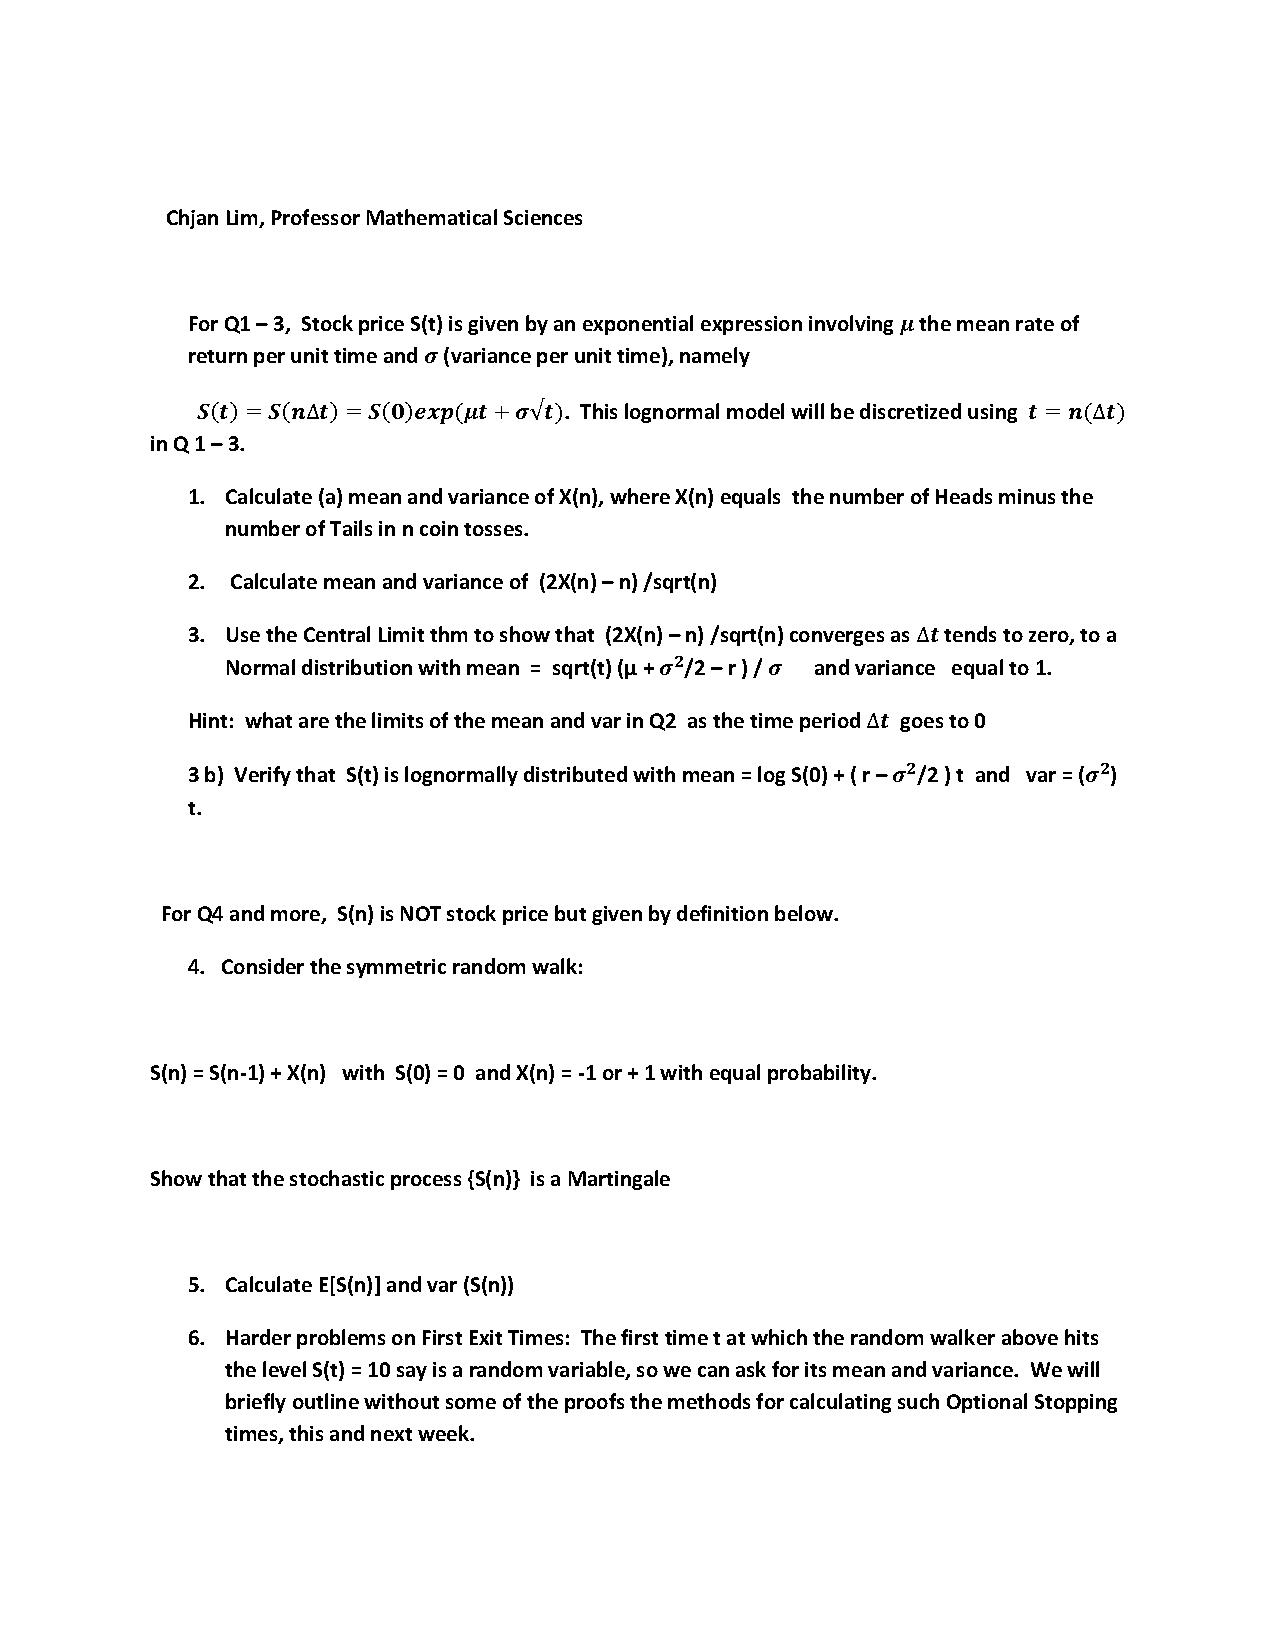
\includepdf[pages={1}]{worksheet216.pdf}


%	\appendix
%%% \section{}
%%% \label{}
%
%%% References
%%%
%%% Following citation commands can be used in the body text:
%%% Usage of \cite is as follows:
%%%   \cite{key}         ==>>  [#]
%%%   \cite[chap. 2]{key} ==>> [#, chap. 2]
%%%
%
%%% References with bibTeX database:
%
%	\section{Reference}
%	\bibliographystyle{elsarticle-num}
%	\bibliography{moptaRefer}
%
%%% Authors are advised to submit their bibtex database files. They are
%%% requested to list a bibtex style file in the manuscript if they do
%%% not want to use elsarticle-num.bst.
%
%%% References without bibTeX database:
%
%% \begin{thebibliography}{00}
%
%%% \bibitem must have the following form:
%%%   \bibitem{key}...
%%%
%
%% \bibitem{}
%
%% \end{thebibliography}

\end{document}



